\section{Diagrama de capas} % (fold)
\label{sec:diagrama_de_capas}

	Cualquier sistema grande se debe dividir en unidades más pequeñas, de modo que las personas puedan trabajar con una cantidad de información limitada, a la vez y de modo que los equipos de trabajo no interfieran con el trabajo de los otros. La gestión del modelo consiste en paquetes y relaciones de dependencia de los paquetes.
	
	Un paquete es, por tanto, una parte de un modelo. Además, cada parte de un modelo debe pertenecer a un paquete. El modelador puede asignar el contenido de un modelo a un conjunto de paquetes. Pero, para ser funcional, la asignación debe seguir un cierto principio racional, tal como funcionalidad común, implementación estrechamente relacionada, y un punto de vista común.
	
	UML no impone una regla para componer los paquetes, pero una buena descomposición en paquetes realzará enormemente la capacidad de mantenimiento del modelo. Pueden ser organizados por la vista, por la funcionalidad, o por cualquier otra base que el modelador elija.
	
	Los paquetes son unidades de organización jerárquica de uso general de los modelos UML, que contienen elementos del modelo al más alto nivel, y además, pueden contener otros paquetes. Si se eligen bien los paquetes, reflejan la arquitectura de alto nivel de un sistema: su descomposición en subsistemas y sus dependencias. Una dependencia entre paquetes resume las dependencias entre los contenidos del paquete.
	
	En nuestro caso, vamos a agrupar los paquetes en base a dos capas. \textbf{La capa específica y la capa genérica. (Figura \ref{fig:acapas})} 
	
	En la primera, se hace mención a los paquetes propios de la aplicación, como son todos aquellos relacionados con las \textit{Actividades de los médicos, de los pacientes, de las fichas médicas, del administrador y de los usuarios genéricos.} Además, todos estos paquetes se dividen en subpaquetes, para agrupar una serie de actividades más específicas de cada uno de ellos. 
	
	Por su parte, en la segunda, se agrupan una serie de paquetes que pueden ser reutilizados en otras aplicaciones. En este proyecto son los relacionados con el \textit{registro de usuarios, algunas librerías javascript, la función autocompletar, la posibilidad de realizar paginación y todo lo relacionado con el multilenguaje.}
	
	\begin{figure}[H]
	  \centering
	    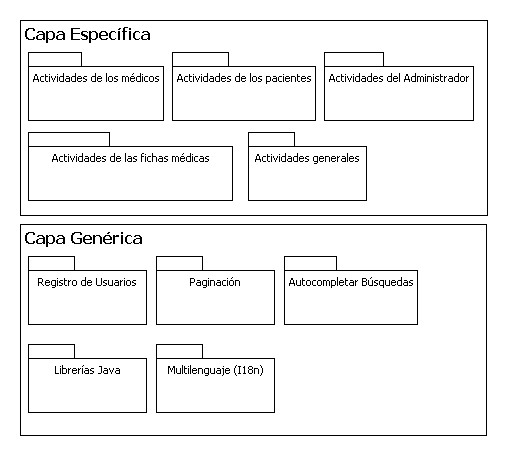
\includegraphics[width=13cm]{img/jpg/acapas/capas.jpg}
	  \caption{Diagrama de Capas}
	  \label{fig:acapas}
	\end{figure}
	
	Una vez visto el diagrama general dividido en dos capas principales, con los subsistemas(paquetes) que contienen cada una de ellas, vamos a ver con más detalle los paquetes de la capa específica.
	
	En primer lugar, el paquete de \textit{Actividades de los médicos} (Figura \ref{fig:acapas_medicos}), que está compuesto por \textit{Gestión del horario, del calendario, de los pacientes, de las plantillas, de las estadísticas y la administración.}
	
	A continuación tenemos los paquetes en los que están divididas las \textit{Actividades de los pacientes} (Figura \ref{fig:acapas_pacientes}), que son \textit{la Gestión del calendario, de los médicos y de las fichas médicas.}
	
	Por último, vemos los paquetes que forman las \textit{Fichas médicas} (Figura \ref{fig:acapas_fichas}). Éstos son \textit{Gestión de antecedentes, de informes, de tratamientos, de exploraciones, de pruebas y de observaciones}.
	
	\begin{figure}[H]
	  \centering
	    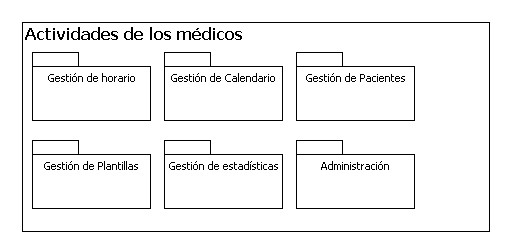
\includegraphics[width=13cm]{img/jpg/acapas/Actividades_medicos.jpg}
	  \caption{Diagrama de Capas}
	  \label{fig:acapas_medicos}
	
	\begin{figure}[H]
	  \centering
	    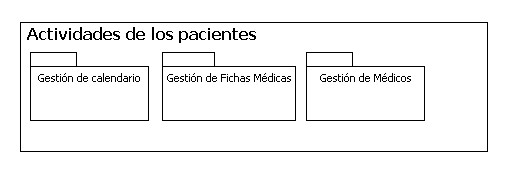
\includegraphics[width=13cm]{img/jpg/acapas/Actividades_Pacientes.jpg}
	  \caption{Diagrama de Capas}
	  \label{fig:acapas_pacientes}
	\end{figure}
	
	\begin{figure}[H]
	  \centering
	    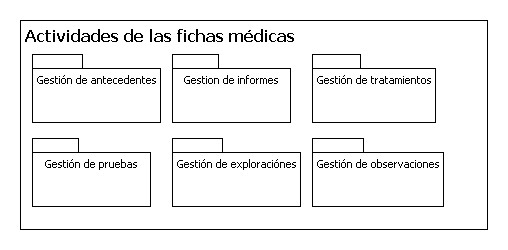
\includegraphics[width=13cm]{img/jpg/acapas/fichas_medicas.jpg}
	  \caption{Diagrama de Capas}
	  \label{fig:acapas_fichas}
	\end{figure}
	\end{figure}

% section diagrama_de_capas (end)
